%!TEX root = ../swiatlow_thesis.tex
\label{chapter:detector}

The design of the LHC, with two high-luminosity interaction points at opposite ends of the ring, called for two general purpose detectors to be built in these locations. Their charge was to accurately reconstruct collision events in the most hostile conditions yet seen in a collider: with a bunch spacing of 25 ns and the unprecedented introduction of pile-up the detectors would have an enormous challenge ahead of them in dealing with both the rate and the reconstruction of events. ATLAS (A Toroidal LHC APparatus)~\cite{ATLASPaper} and CMS (Compact Muon Solenoid)~\cite{CMSPaper} were the two detectors built for this task, with ATLAS occupying the (much more convenient) Point 1 and CMS located at the (very distant) Point 5. The data presented in this thesis was collected by the ATLAS experiment in $pp$ collisions at $\sqrt{s} = 8$~TeV in 2012. 


\editnote{Paragraph on general principles?}


Particle detectors measure particles via their interactions with matter, as drawn schematically in Figure~\ref{fig:detector:schematic}. For example, charged particles (such as electrons and some hadrons) interact electromagnetically with silicon and gas tubes, leaving hits in different layers of detectors which can be traced back to form a track. Electrons and photons, with their low masses and high rate of interaction with matter, are measured by the electromagnetic calorimeter. The calorimeter is composed of alternating layers of metal meant to cause the particle to interact and lose energy, and active materials which measure the energy left behind in these interactions. The hadron calorimeter follows a similar principle, and alternately placed layers of metal and active material again aim to stop and measure the hadrons which the electromagnetic calorimeter did not stop. Muons, which do not interact very much with matter most matter but do leave hits in trackers, survive past even the hadronic calorimeter, and a special set of muon detectors can be used to identify them there. Neutrinos, as they interact with matter only via the weak force and thus very rarely, escape detection and are reconstructed only by inferring their presence from the lack of momentum conservation in the transverse plane. \editnote{this isn't great?}


%%%%%%%%%%%%%%%%

\begin{figure}
\centering
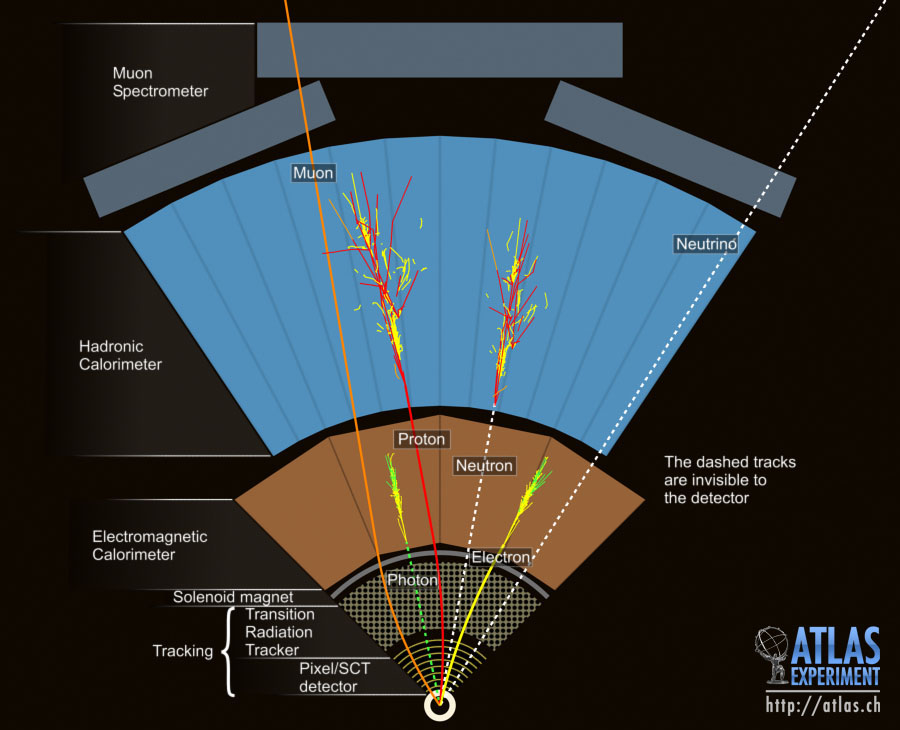
\includegraphics[width=0.7\textwidth]{schematic.jpg}
\label{fig:detector:schematic}
\caption{A schematic diagram of the interactions of various particles with detector components. Copyright CERN.}
\end{figure}

%%%%%%%%%%%%%%%% 

General purpose particle detectors thus demand the following characteristics: \editnote{define radiation lengths? above?}

\begin{enumerate}
	\item Tracking systems must be able to identify primary and secondary vertices, while minimizing the radiation lengths before the calorimeters
	\item Strong calorimetry systems are required to accurately measure the energy and position electrons, photons, and hadrons
	\item Muon systems must be able to precisely reconstruct muons
\end{enumerate}

To this end, the ATLAS detector is built in the traditional onion-layer configuration, which measures particles as they travel perpendicular to the beam. The Inner Detector, composed of the concentric Pixel, SCT \editnote{define}, and Transition-Radiation-Tracker (TRT) subsystems, lies at the center of the detector and precisely measures tracks created by charged particles. A 2 T solenoid encloses the Inner Detector, bending charged particles and enabling the measurement of their momenta. Next the Electromagnetic Calorimeter (ECal), composed of liquid argon (LAr) and copper, sits outside of the solenoid in a liquid nitrogen cryostat, and measures energy deposits from electrons and photons (as well as hadrons to a lesser extent). The Hadronic Calorimeter, built to measure and stop any remaining hadronic particles, is composed of steel and scintillating tile in the center (referred to as the barrel), and LAr and copper in forward regions (referred to as end-caps). Surrounding these are an additional set of magnets: the superconducting air-core toroids of the barrel and endcaps, which bend particles in the plane perpendicular to that of the bending due to the solenoid. \editnote{That needs cleaning.} The Muon Spectrometer (composed of MDT, RPC, TGC, and CSC subsystems) sits outside of (and next to) these magnets, and provides a final measurement of the charged particles which reach that far. The entire detector is shown in Figure~\ref{fig:detector:atlas}. The incredible size of the detector-- 25 m in diameter, and 46 m long-- is dominated by the Muon Spectrometer and the toroids. On the other hand, the detector is comparatively light (only 7000 tons, compared to 14,000 tons for CMS), as the air-core toroids do not add substantial weight to the detector. \editnote{decide how to cite all this}


%%%%%%%%%%%%%%%%

\begin{figure}
\centering
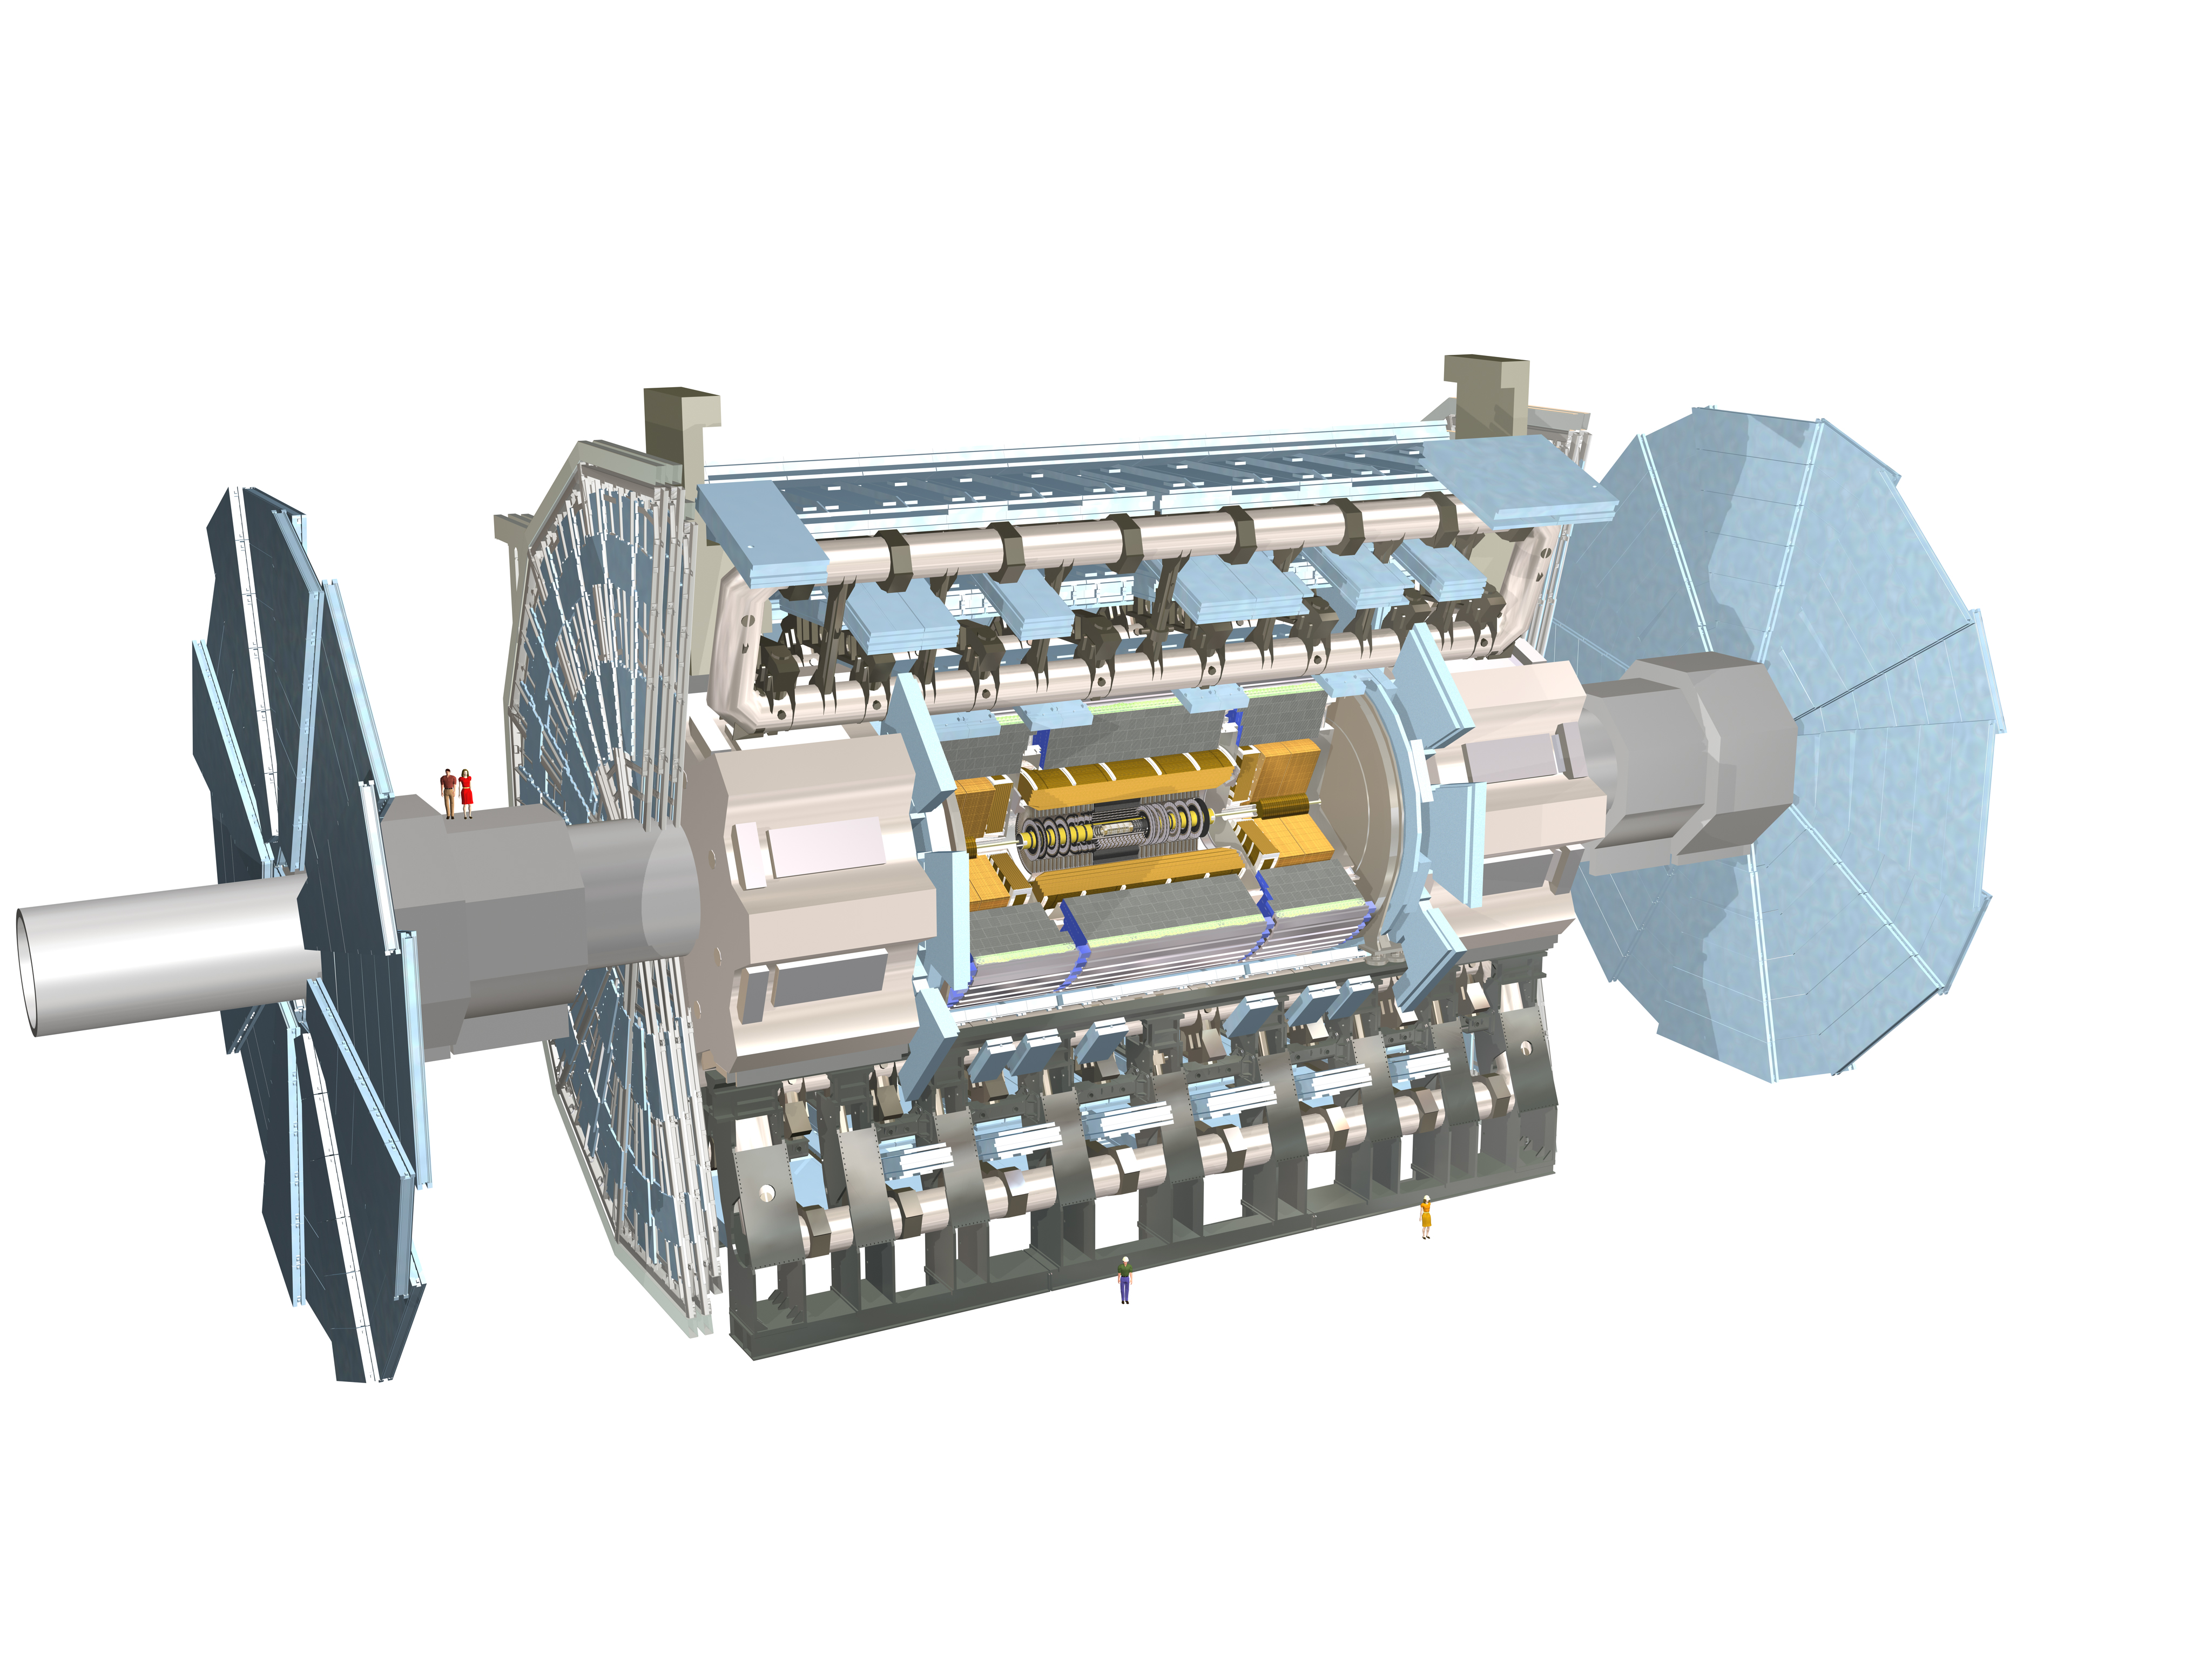
\includegraphics[width=0.85\textwidth]{atlas.jpg}
\label{fig:detector:atlas}
\caption{A computer-generated view of the ATLAS detector, with people for scale. Copyright CERN.}
\end{figure}

%%%%%%%%%%%%%%%% 


In keeping with the principle of ``similar, but opposite'' established by their locations, the ATLAS and CMS detectors take complementary approaches to the various aspects of event reconstruction in collisions. All general purpose detectors have the same basic goals: the must reconstruct the outgoing, stable particles produced in collisions and the subsequent decays of particles in these collisions. Different particles are detected with different general classes of detectors, of which there are many possible types. For example, electrons and photons are measured by the ECal, for which ATLAS used a liquid argon (LAr) and copper system while CMS used a crystal lead tungstate system. Each had their own advantages and disadvantages (ATLAS's was less costly and already proven technology with better position resolution, while CMS took a riskier route which promised better energy resolution), but overall performance between the detectors tends to be very similar because of various trade-offs. In the case of the ECals, the precision of ATLAS and CMS's $H\rightarrow \gamma \gamma$ measurements ended up being largely similar \editnote{cite?}, in no small part because CMS's all-silicon tracking system introduced greater radiation lengths before the calorimeters, thereby prompting more photons to convert and losing precision in the measurement. On the other hand, CMS's comparatively weak brass hadronic calorimeter (compared to ATLAS's higher resolution tile calorimeter), is compensated by their tracking system, which enables a particle-flow reconstruction algorithm to combine information from all detectors and improve jet performance to levels very similar to ATLAS. \editnote{consider citations, and substantial revisions here}. Similarly, the large size and extra toroid magnets of ATLAS allow for a larger lever-arm and an additional set of measurements of muons (enabling reconstruction with or without the inner detector): however, muon reconstruction performance in CMS is very similar because the stronger solenoidal magnetic field (4 T compared to 2 T) allows for a better measurement using the inner detector only (with the muon systems on CMS providing only a tag of a passing muon, and not a complete reconstruction). 


%2012 luminosity figure? Or in LHC section?



%Detector figure

\section{History}

The first public discussion of the proposals which became the ATLAS detector occurred in 1992 at the General Meeting on LHC Physics at Evian-les-Bains~\cite{Evian,EvianCourier}. At the time, four general purpose detectors (much like the four detector configuration in place at LEP) were seriously considered: EAGLE, ASCOT, CMS, and L3 (as an upgrade to the existing LEP detector, including a movable stage which would allow it to take data from both $e^+/e^-$ and $pp$ collisions). Several additional single purpose (heavy ion, neutrino, and $B$-physics) detectors were also proposed.

ATLAS emerged in a later 1992 Letter of Intent as a merger of the ASCOT and EAGLE collaborations~\cite{ATLAS-LoI}. ASCOT (Apparatus with SuperCOnducting Toroids) contributed the physically-defining feature of the secondary toroidal magnet system and standalone muon measurement system, as well as the tradition of using a tortured amalgamation of letters to form a name. EAGLE (Experiment for Accurate Gamma, Lepton and Energy measurements) on the other hand featured a stronger 2 T magnetic field, and inner-detector and calorimeter designs more similar to some of the final ATLAS systems. The detector described in the Letter of Intent already resembled ATLAS in many important ways, featuring the superconducting air-core toroids, accordion-shaped liquid Argon electromagnetic calorimeters, scintillating tile hadron calorimeters, and multi-design inner detector. \ref{fig:detector:earlyatlas} shows an early drawing of ATLAS from the Letter, and already the detector looks recognizable to its current form.

% Any citations on UA1 origins?

%%%%%%%%%%%%%%%%

\begin{figure}
\centering
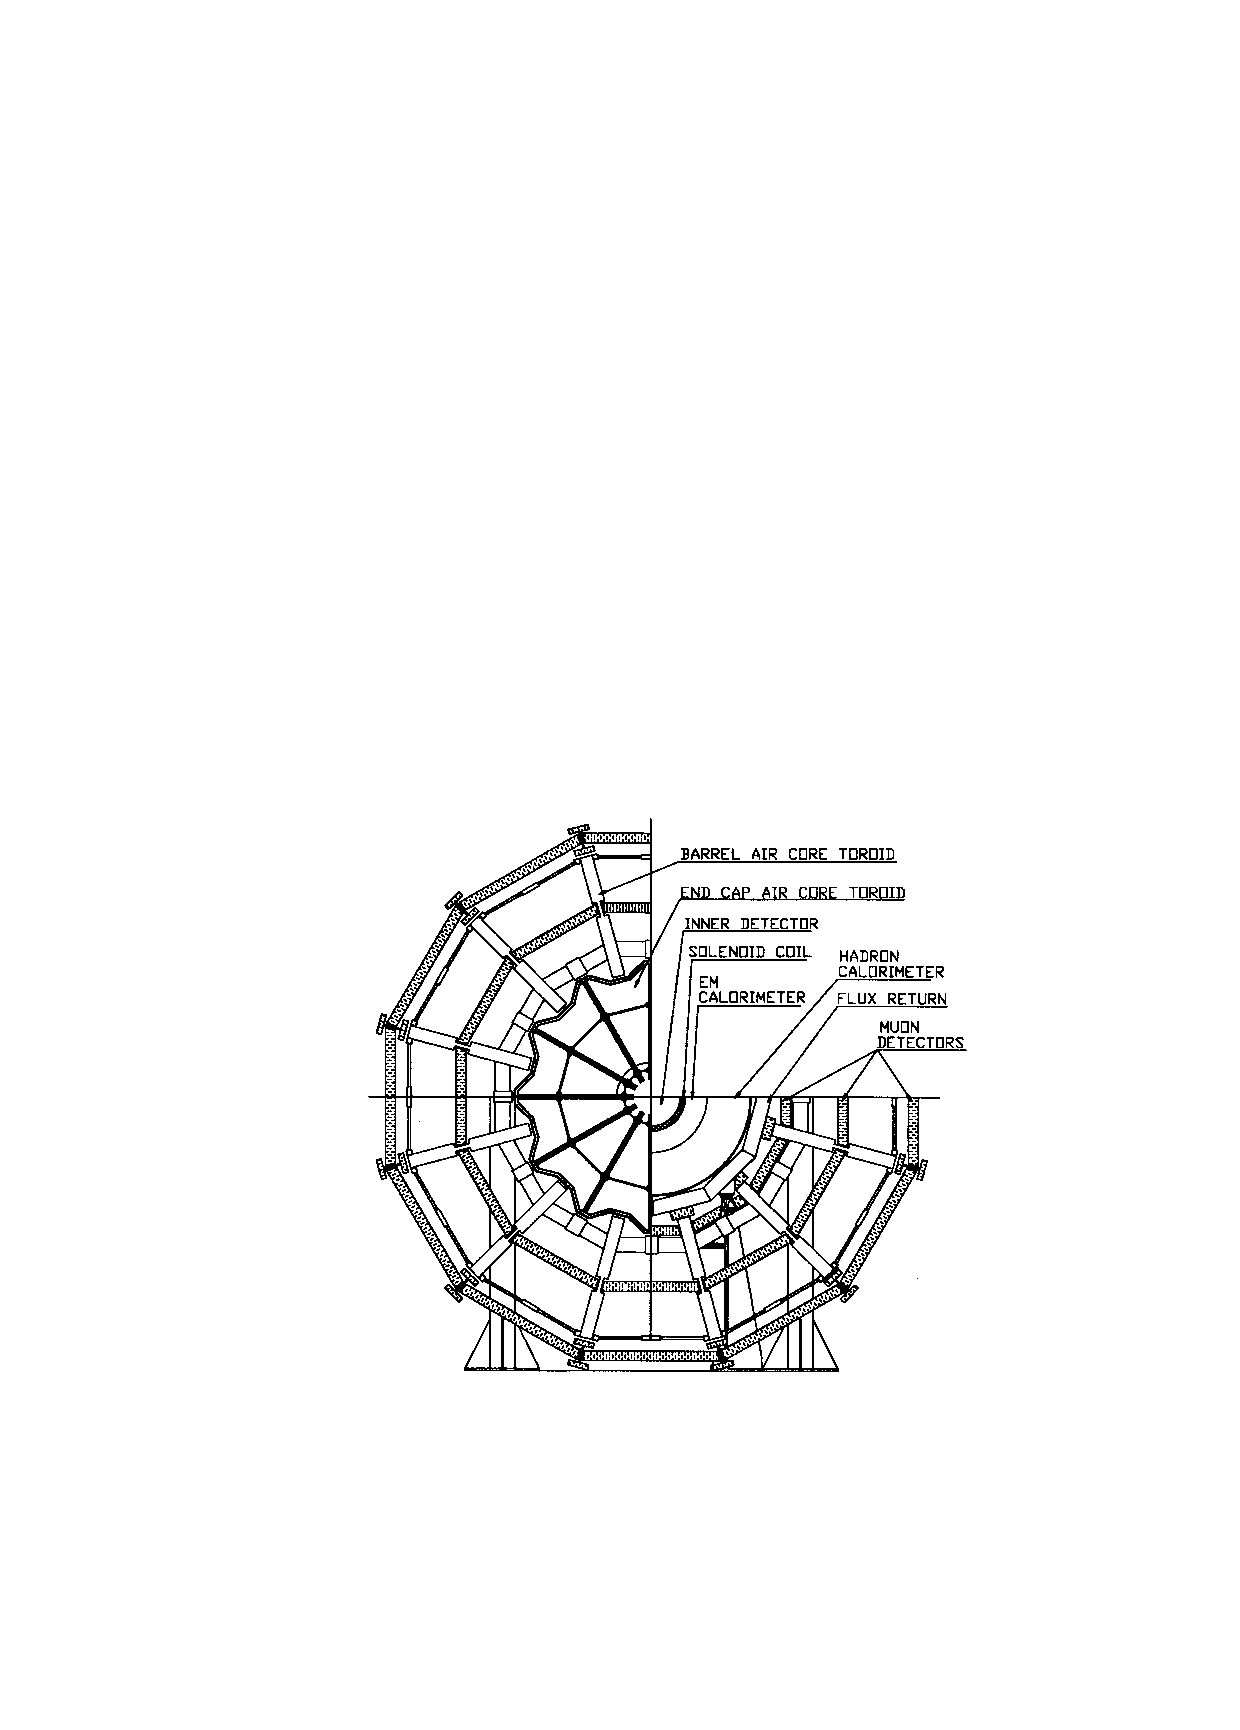
\includegraphics[width=0.7\textwidth]{early-atlas.pdf}
\label{fig:detector:earlyatlas}
\caption{An early view of a potential superconducting air-core toroid magnet system for the ATLAS detector from the 1992 Letter of Intent~\cite{ATLAS-LoI}.}
\end{figure}

%%%%%%%%%%%%%%%% 


% approval dates

% cavern construction (picture?)

% construction milestones

% first data, first papers

% quenching? higgs discovery


\section{Magnet Systems}

\subsection{Solenoid}

%%%%%%%%%%%%%%%%

\begin{figure}
\centering
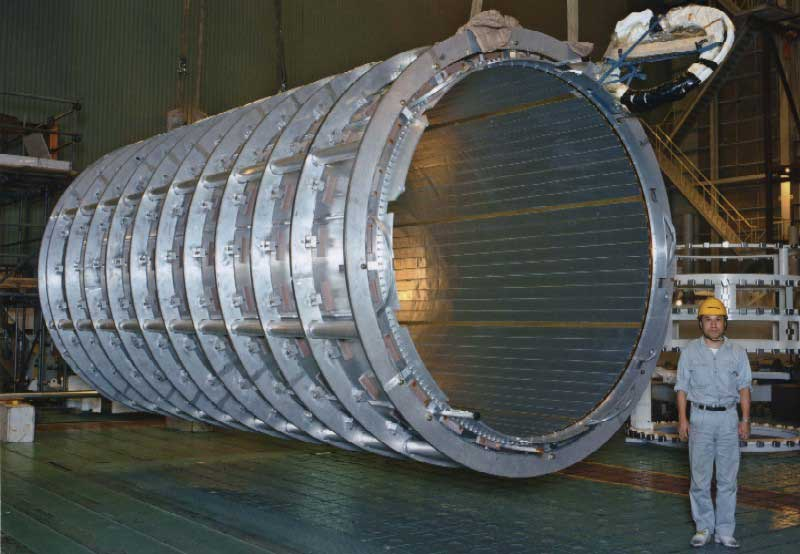
\includegraphics[width=0.7\textwidth]{solenoid.jpg}
\label{fig:detector:solenoid}
\caption{A photograph of the ATLAS solenoid shortly after the winding of the coils was finished. Copyright CERN.}
\end{figure}

%%%%%%%%%%%%%%%% 


\subsection{Toroids}


%%%%%%%%%%%%%%%%

\begin{figure}
\centering
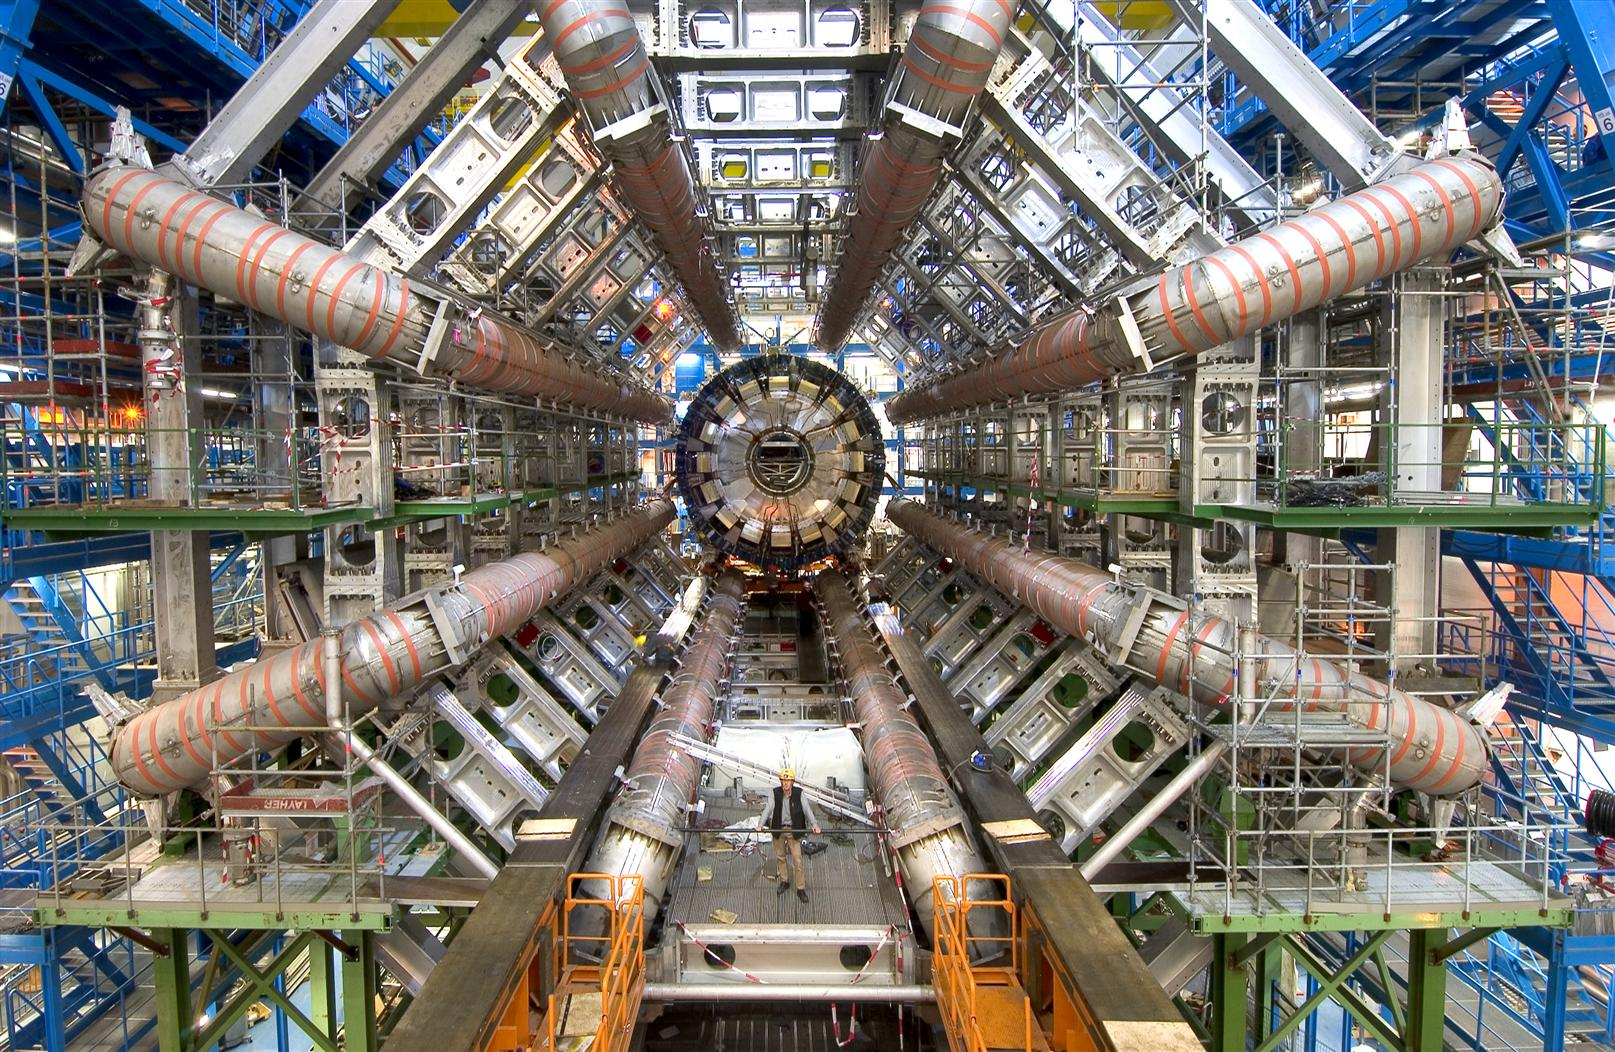
\includegraphics[width=0.7\textwidth]{toroid.jpg}
\label{fig:detector:solenoid}
\caption{A photograph of the ATLAS barrel toroids after their installation. Note person in the center for scale. Copyright CERN.}
\end{figure}

%%%%%%%%%%%%%%%% 



%%%%%%%%%%%%%%%%

\begin{figure}
\centering
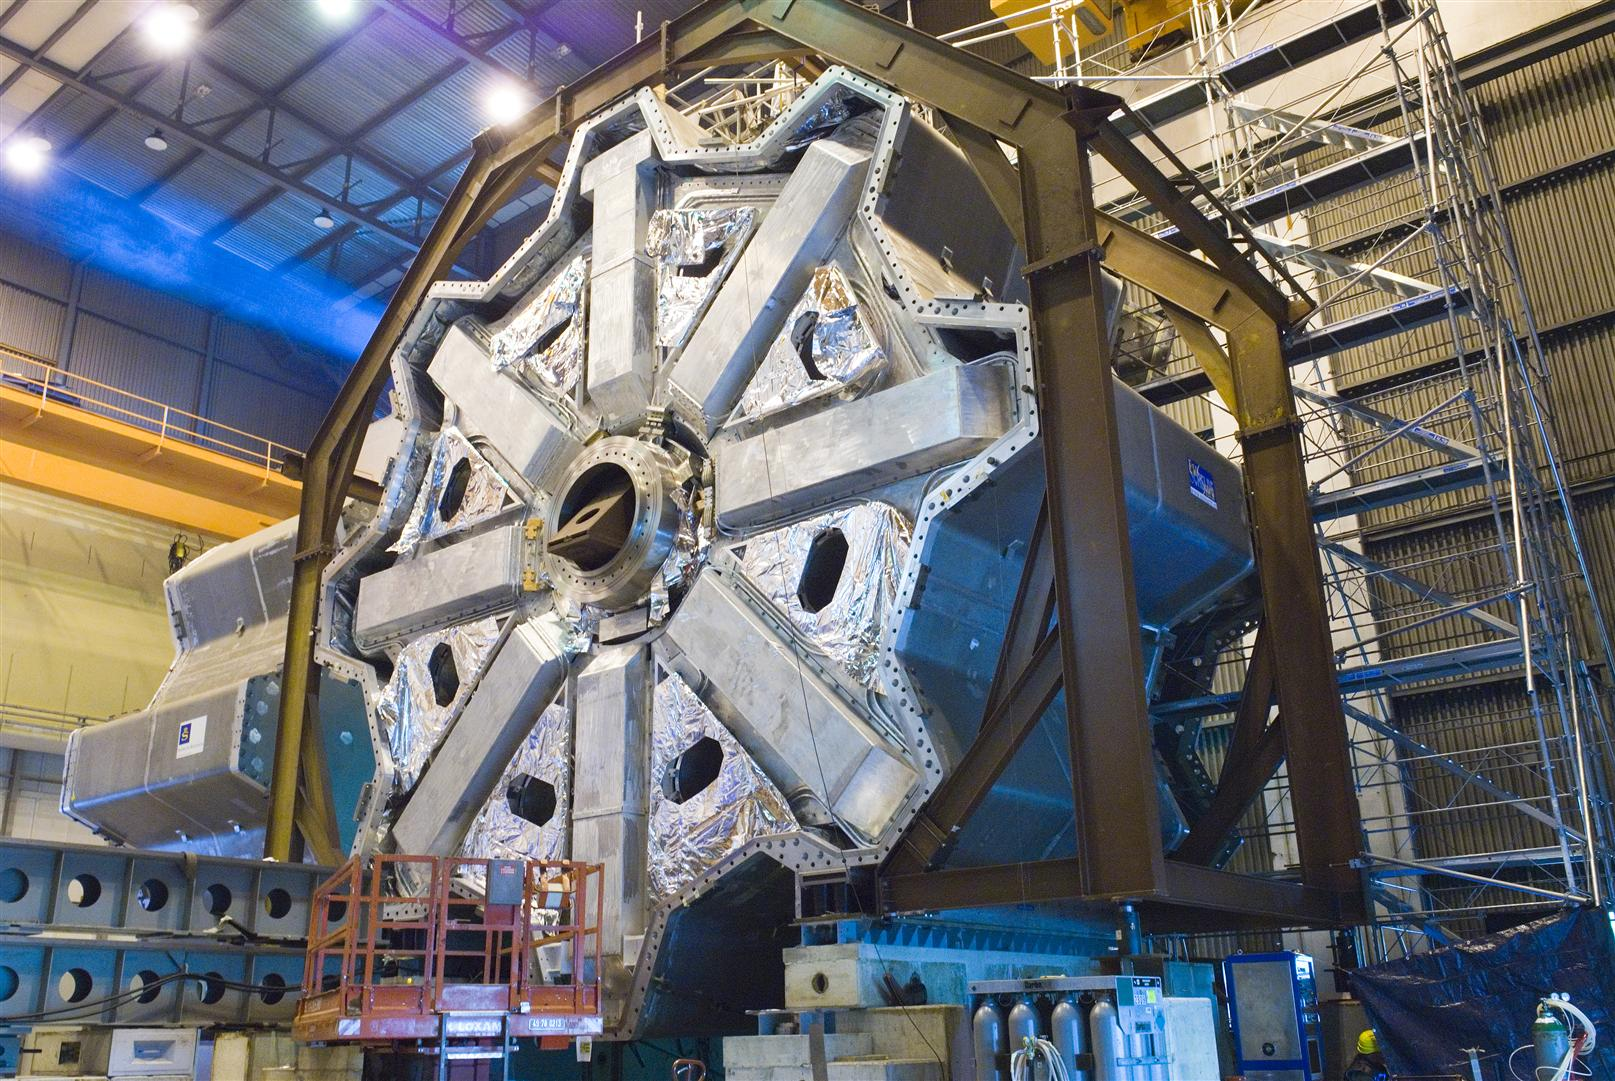
\includegraphics[width=0.7\textwidth]{endcap-toroid.jpg}
\label{fig:detector:solenoid}
\caption{A photograph of an ATLAS endcap toroid shortly before its installation in the detector. Copyright CERN.}
\end{figure}

%%%%%%%%%%%%%%%% 


\section{Inner Detector}


Define ID

At design luminosity, the detector is expected to measure approximately 1000 charged particles every 25 ns within the detector acceptance.

%%%%%%%%%%%%%%%%

\begin{figure}
\centering
\includegraphics[width=0.7\textwidth]{inner-detector.jpg}
\label{fig:detector:inner-detector}
\caption{A computer-generated view of the ATLAS inner detector, with relevant sizes of the detector marked out. Copyright CERN.}
\end{figure}

%%%%%%%%%%%%%%%% 

%%%%%%%%%%%%%%%%

\begin{figure}
\centering
\includegraphics[width=0.7\textwidth]{inner-detector-2.jpg}
\label{fig:detector:inner-detector-2}
\caption{A cut-out view of the ATLAS inner detector, showing the layers a particle would interact with as it passed outward from the collision point. Copyright CERN.}
\end{figure}

%%%%%%%%%%%%%%%% 

\subsection{Silicon Pixel Detector}

The innermost ATLAS sub-detector is the Silicon Pixel Detector~\cite{ATLASPaper}. The principal of detection for the pixel detector follows the standard ionizing radiation detector~\cite{Detectors}. Charged particles interact with the active medium (doped silicon), knocking electrons loose from their host atoms and creating electron-hole pairs. An applied voltage carries the holes and electrons to opposite ends of the detectors, where they are read out. The active regions are very small in both $x$ and $y$ dimensions, allowing for many independent measurement channels in a small area. Given the high number of particles expected from LHC collisions, and that the density is greatest nearest to the interaction point, it is critical that the innermost detector have a huge number of very small channels, making the task perfectly suited for a pixel detector.

80.4 million independent pixel channels, with a size of $50 \times 400~\mu$m, are read out by 1744 bump-bonded modules attached to the active sensors. Each of the modules are composed of 16 front-end chips~\cite{ATLASPaper}. This corresponds to a combined active area of 1.7 $m^2$. The detector is arranged in three radial layers in the barrel section, and three disks in the end-caps. In the radial layers, the pixels have a resolution of $10 \times 115~\mu$m in $R-\phi$ and $z$ respectively, and in the end-caps the orientation is perpendicular and the resolution is $10 \times 115~\mu$m in $R$ and $R-\phi$: the orientations are always chosen such that the most precise measurement takes place in the direction most relevant to the measurement of the track $p_T$.\footnote{The $R-\phi$ coordinate is simply a distance-projected version of the azimuthal angle $\phi$.} The barrel and disk arrangement is shown in Figure~\ref{fig:detector:pixel}. Hits are read out when charge has been collected over a tunable threshold determined by the noise of each pixel, resulting in typical occupancies of $10^{-4}$ -- $10^{-5}$, though this grows obviously grows with additional $pp$ interactions.

The innermost radial layer, known as the $b$-layer, sits only 50.5 mm from the center of the beampipe, while the outermost layer is located at 122.5 mm~\cite{ATLASPaper}. By placing detectors so close to the interaction point, it is possible to very accurately measure the location of both  primary vertices-- the locations of $pp$ collisions-- and second vertices-- the locations of the displaced decays of particles with long lifetimes, such as $B$-hadrons~\cite{ATLASExpected}.

Placing the detector so close to the beamline comes at a price, however, as the detector is particularly susceptible to radiation damage due to the high flux of particles through a small area. At design luminosity, this is expected to be about 158 kGy/year at the $b$-layer, reduced to 25.4 kGy/year at the outermost layer~\cite{ATLASPaper}. Damage comes in the form of displaced atoms in the doped silicon lattice, resulting in lower electron-hole yields per particle interaction. Some of the damage is mitigated by operating at cold temperatures (typically $-5$ to $-10$\degree~C), and higher bias voltages can also alleviate the effects.

While the entire Inner Detector is expected to be replaced after 300 \ifb~are collected in order to replace the damaged components, the long shutdown of 2013-2015 presented ATLAS with the opportunity to augment the existing pixel detector with the so-called Insertable B-Layer (or IBL)~\cite{ATLASIBL}. The IBL, which adds an additional layer of pixels to the barrel and endcap pixel systems, is attached directly to a new carbon-fiber beampipe, and is located only 33 mm from the center of the beampipe. Due to this extremely close distance, the pixel size has been further reduced to $50 \times 250 \mu$m. The vertexing performance (especially secondary vertex identification for $b$-tagging) of ATLAS in Run 2, starting in 2015, is expected to substantially increase due to the IBL. 

%%%%%%%%%%%%%%%%

\begin{figure}
\centering
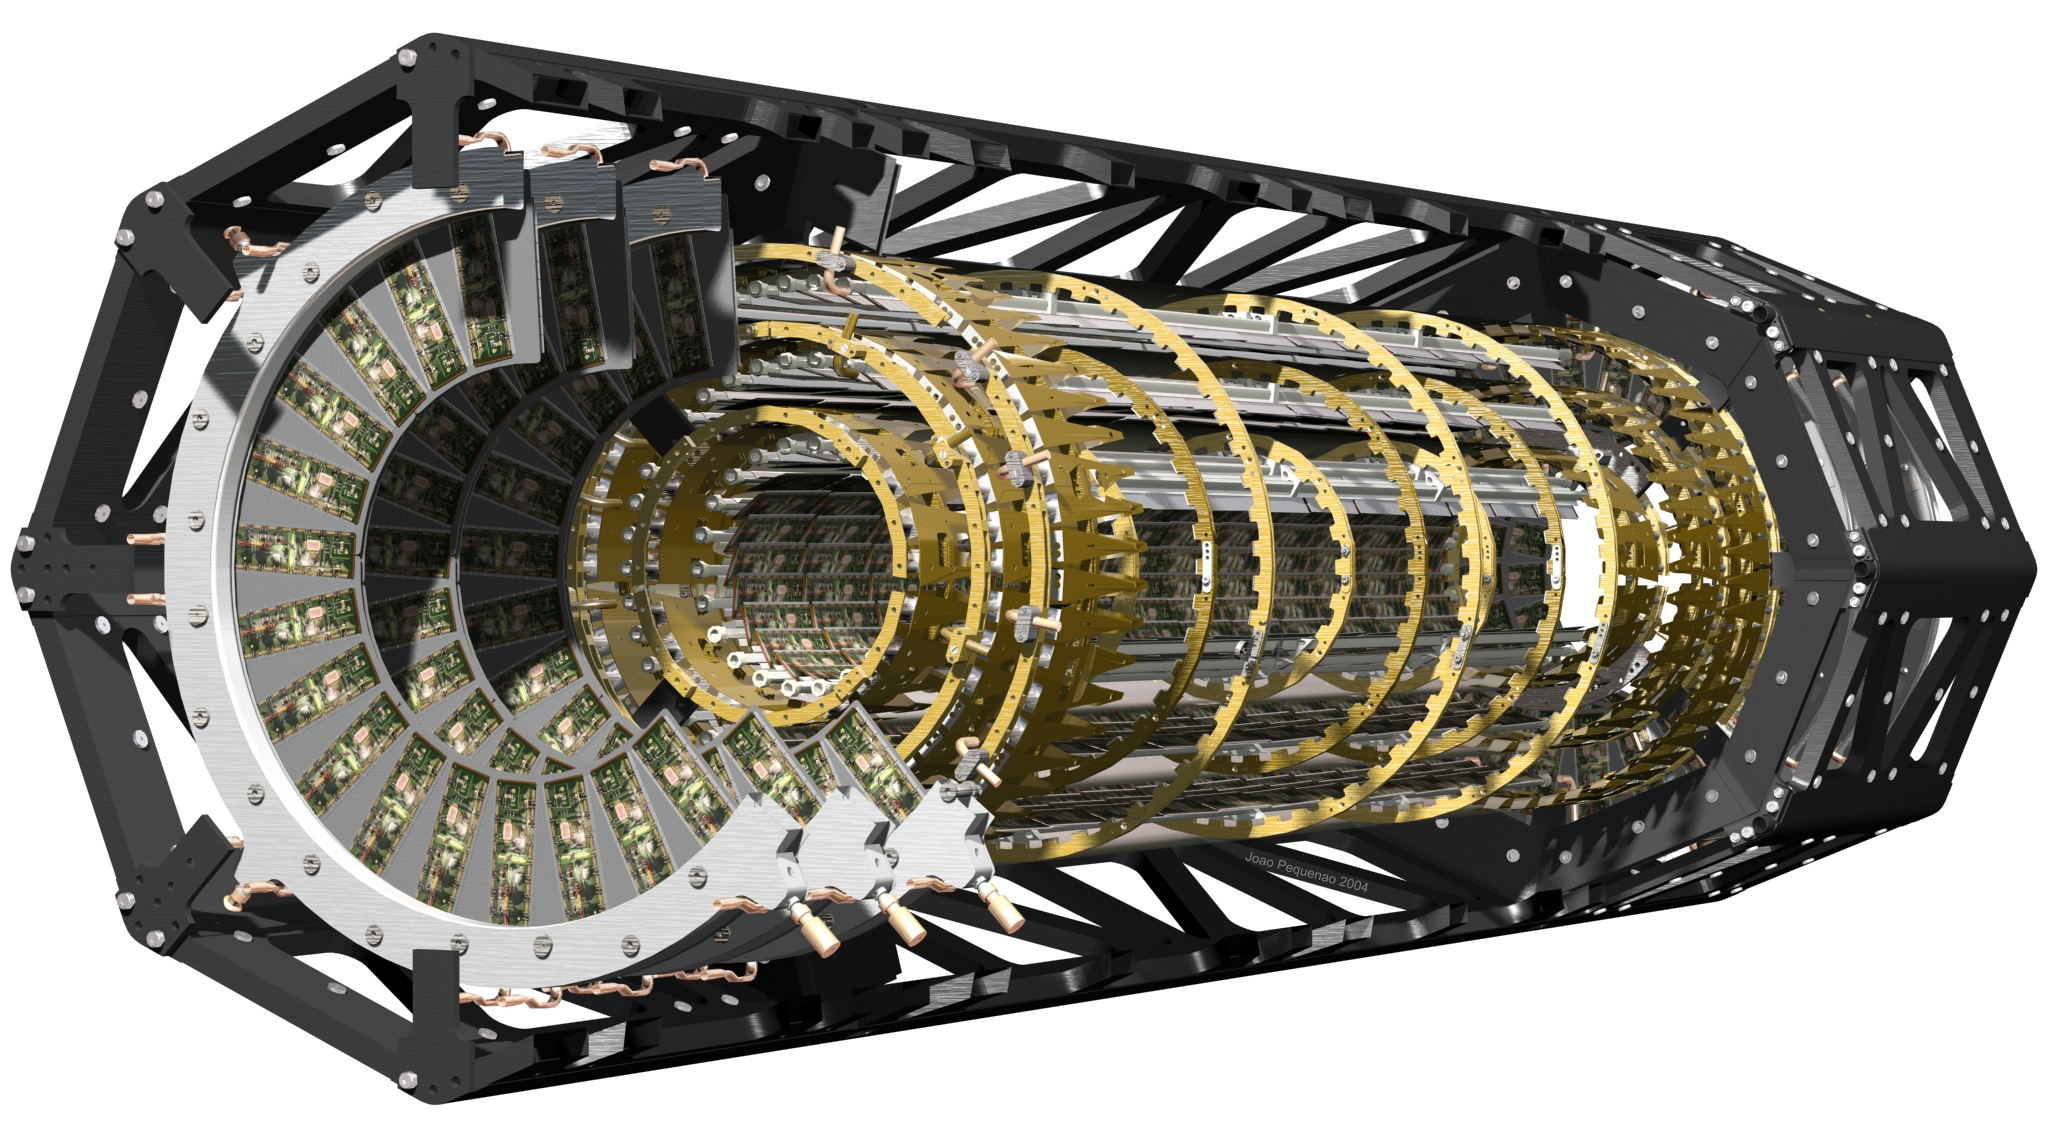
\includegraphics[width=0.7\textwidth]{pixel.jpg}
\label{fig:detector:pixel}
\caption{A computer-generated view of the ATLAS pixel detector. Copyright CERN.}
\end{figure}

%%%%%%%%%%%%%%%% 



\subsection{Silicon Strip Tracker}

The next outermost subdetector in the ID is composed of silicon microstrip (SCT) layers~\cite{ATLASPaper}. 


%%%%%%%%%%%%%%%%

\begin{figure}
\centering
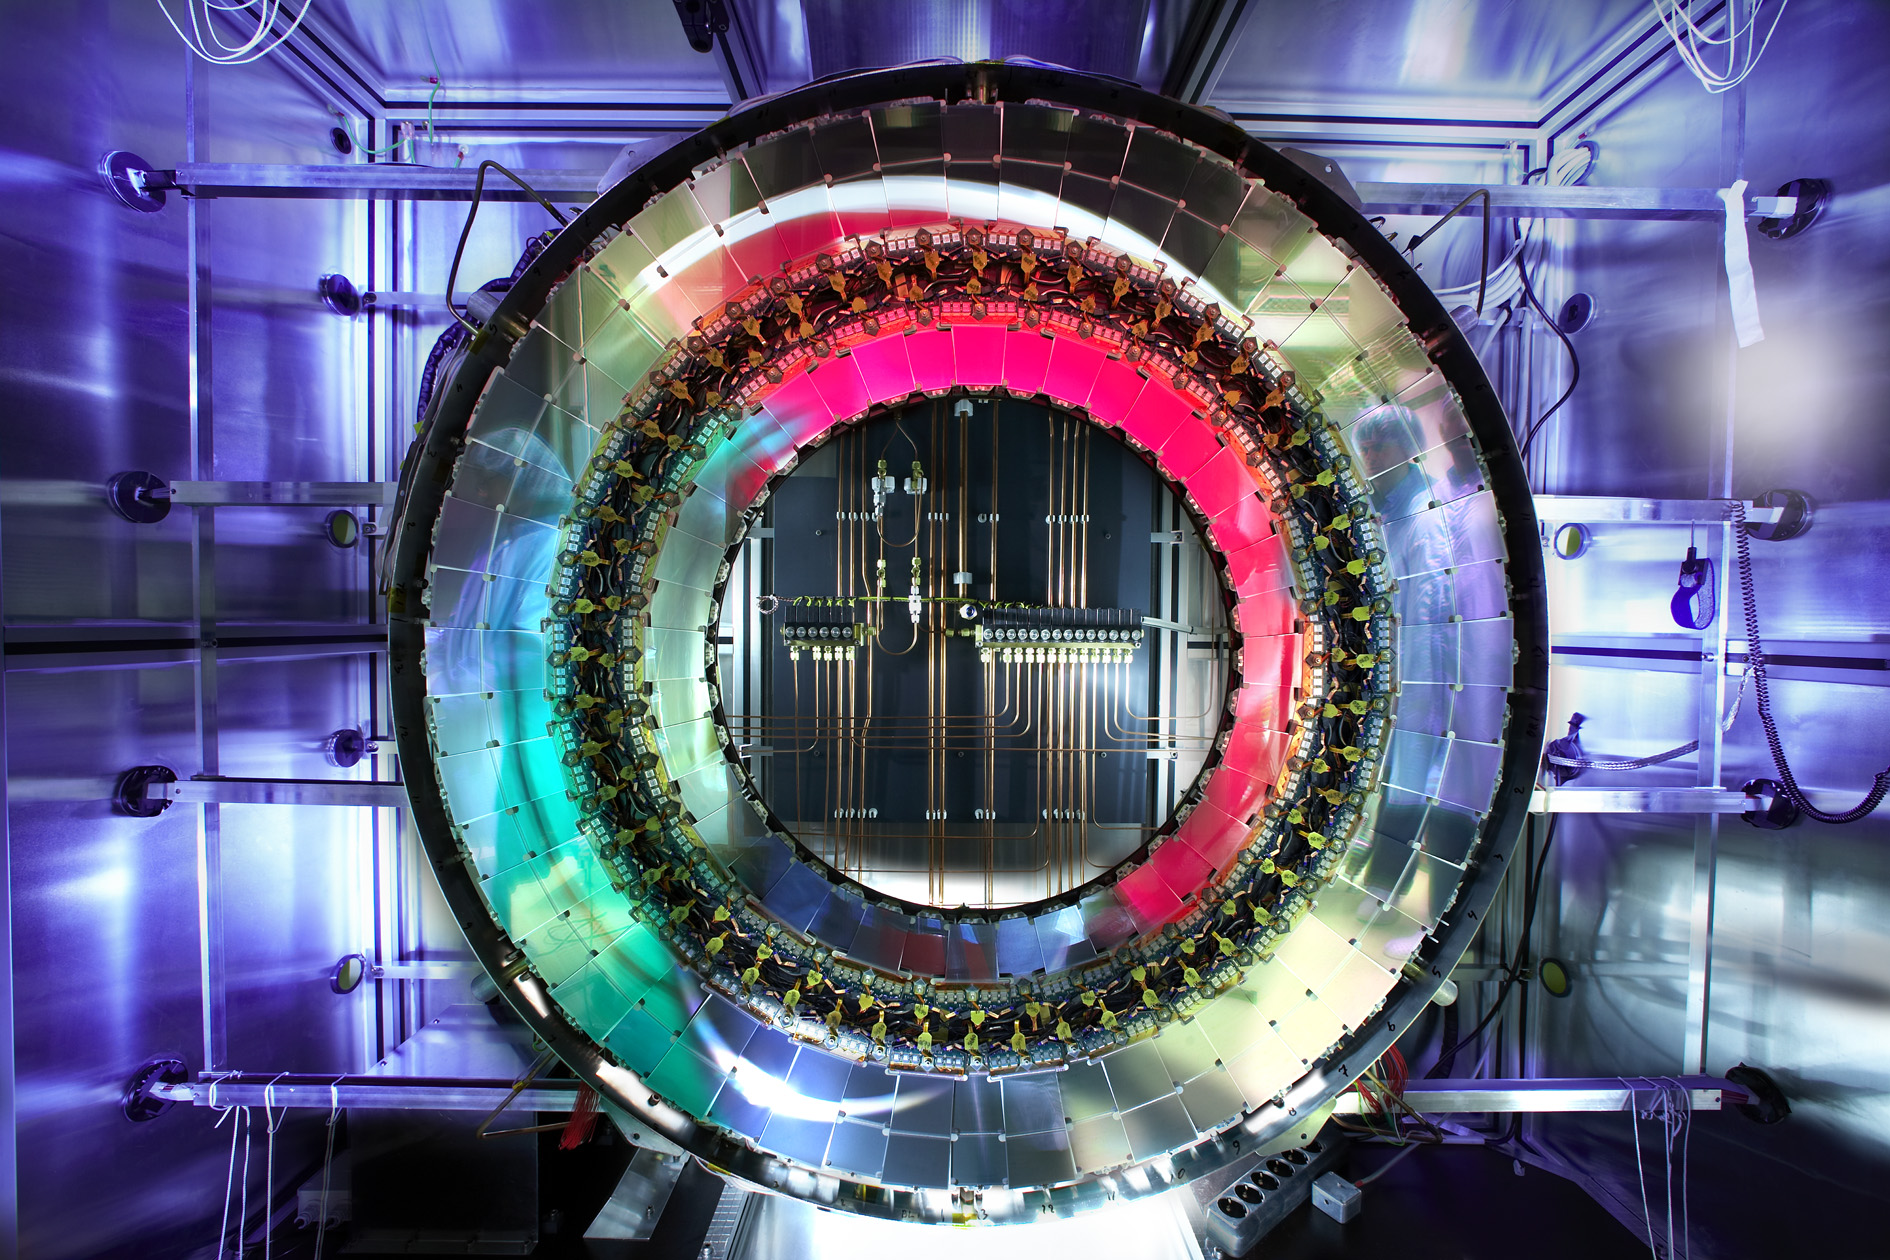
\includegraphics[width=0.7\textwidth]{sct.jpg}
\label{fig:detector:sct}
\caption{A photograph of one segment of the ATLAS SCT end-cap disks. Copyright CERN.}
\end{figure}

%%%%%%%%%%%%%%%% 

\subsection{Transition Radiation Tracker}

%%%%%%%%%%%%%%%%

\begin{figure}
\centering
\includegraphics[width=0.7\textwidth]{trt.jpg}
\label{fig:detector:trt}
\caption{A photograph of the ATLAS TRT system during testing. Copyright CERN.}
\end{figure}

%%%%%%%%%%%%%%%% 

\section{Calorimeters}

%%%%%%%%%%%%%%%%

\begin{figure}
\centering
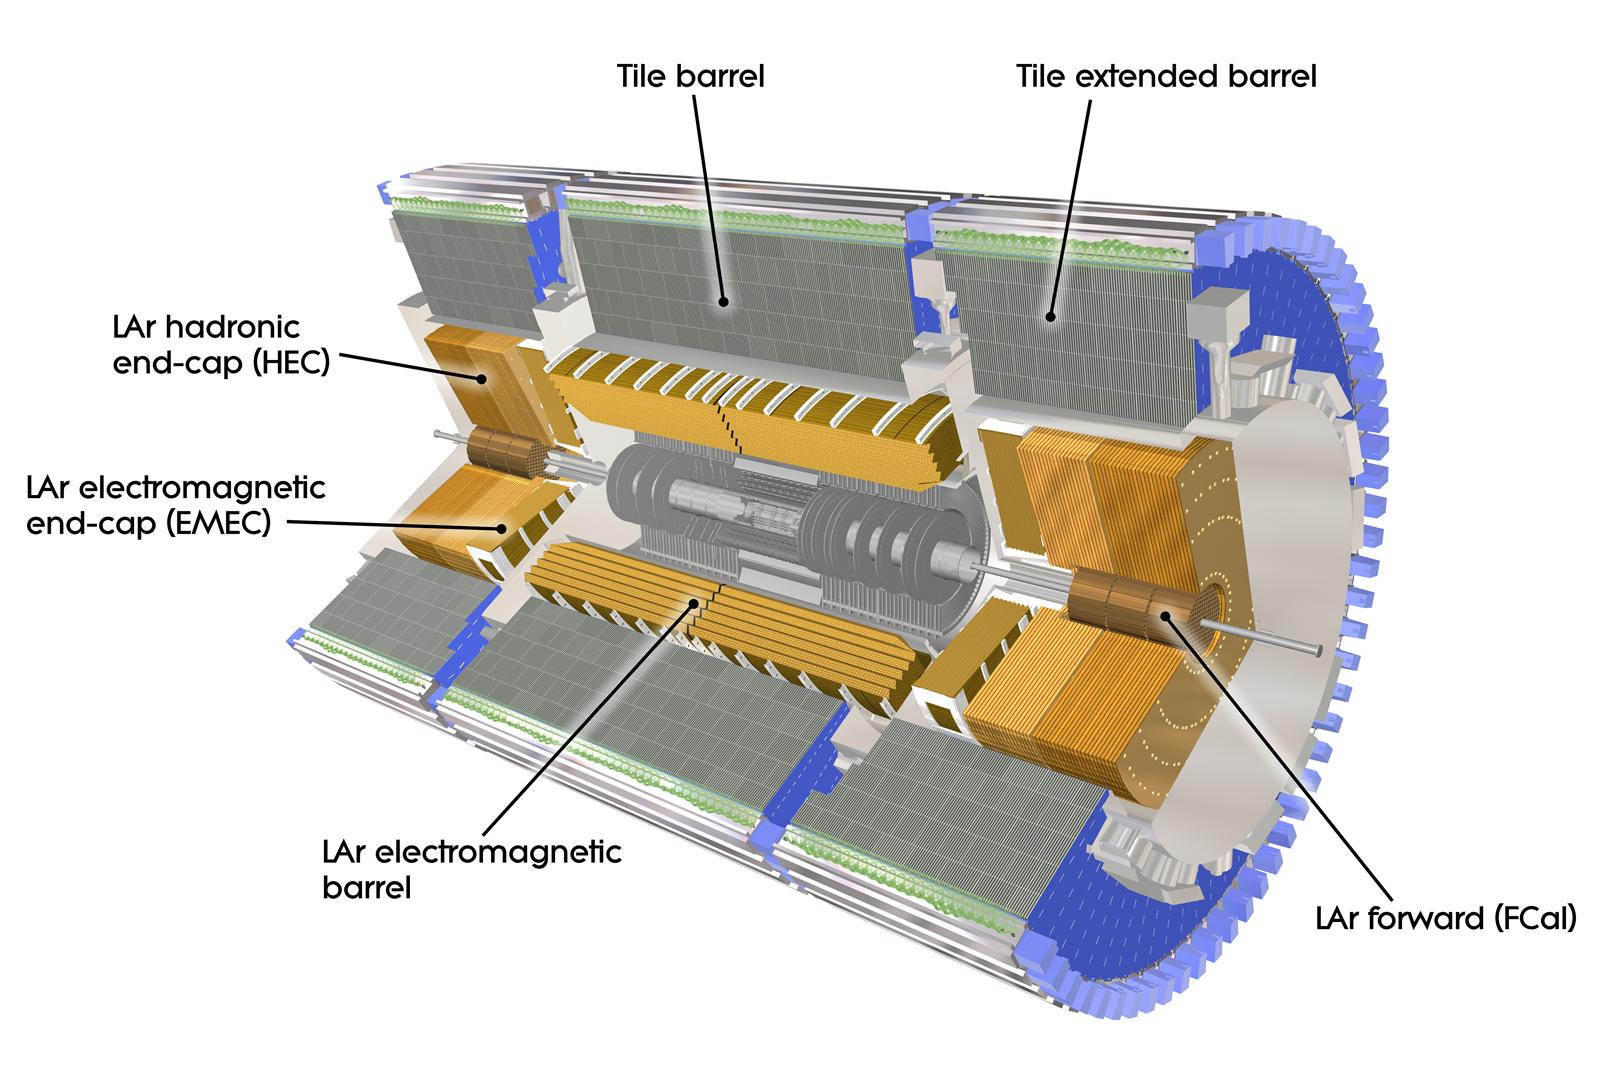
\includegraphics[width=0.7\textwidth]{calorimeters.jpg}
\label{fig:detector:trt}
\caption{A computer generated image of the ATLAS calorimeter system, showing the locations of each different subdetector. Copyright CERN.}
\end{figure}

%%%%%%%%%%%%%%%% 


\subsection{Electromagnetic Calorimeter}

%%%%%%%%%%%%%%%%

\begin{figure}
\centering
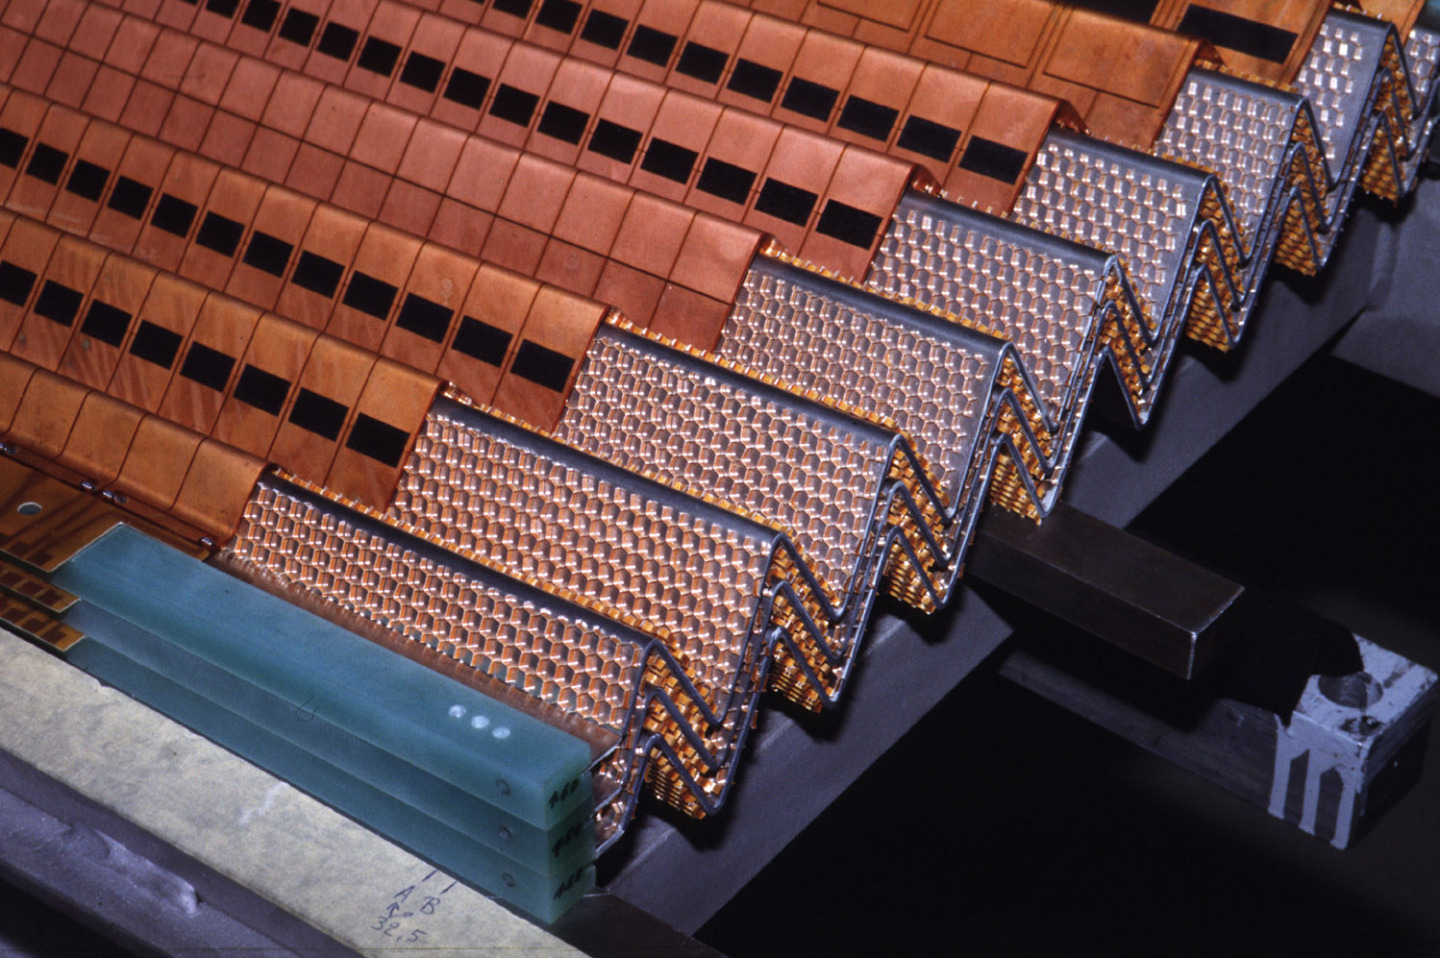
\includegraphics[width=0.7\textwidth]{lar-accordion.jpg}
\label{fig:detector:trt}
\caption{A photograph of the accordion structure used in the LAr barrel. Copyright CERN.}
\end{figure}

%%%%%%%%%%%%%%%% 

%%%%%%%%%%%%%%%%

\begin{figure}
\centering
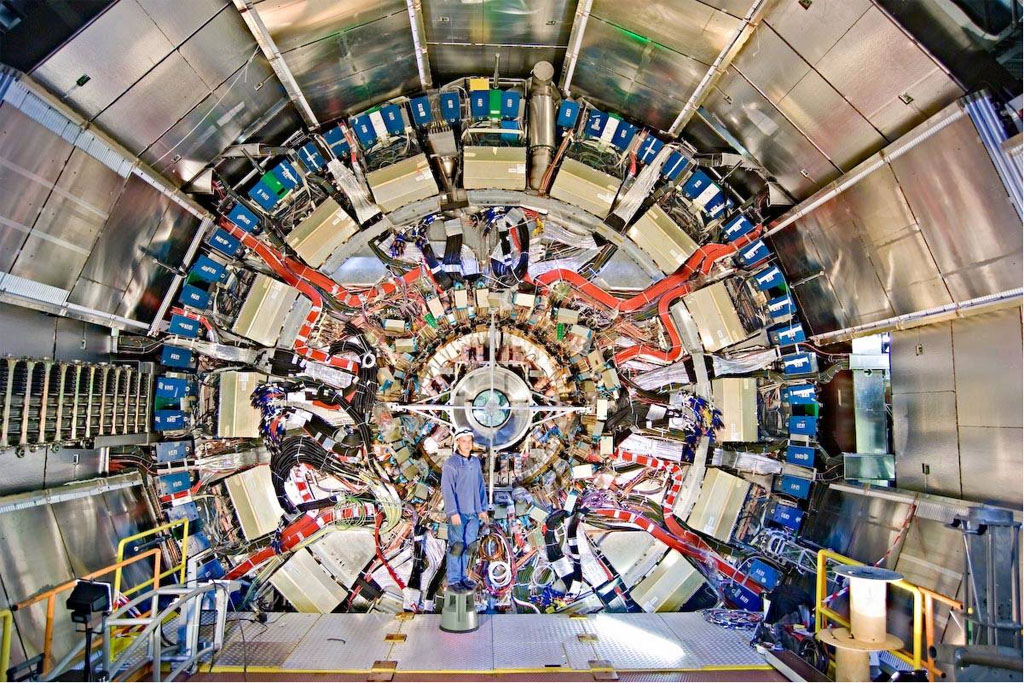
\includegraphics[width=0.7\textwidth]{lar-endcap.jpg}
\label{fig:detector:trt}
\caption{A photograph of the LAr endcap after installation in the cryostat system. Copyright CERN.}
\end{figure}

%%%%%%%%%%%%%%%% 

\subsection{Hadron Calorimeter}

%%%%%%%%%%%%%%%%

\begin{figure}
\centering
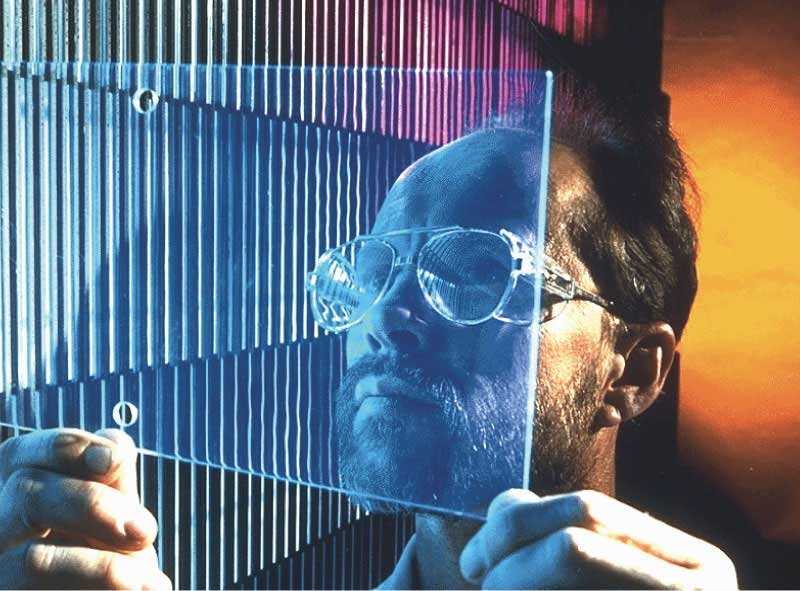
\includegraphics[width=0.7\textwidth]{tile-actualtile.jpg}
\label{fig:detector:trt}
\caption{A photograph of one of the scintillating tiles which give the tile calorimeter its name. Copyright CERN.}
\end{figure}

%%%%%%%%%%%%%%%% 

%%%%%%%%%%%%%%%%

\begin{figure}
\centering
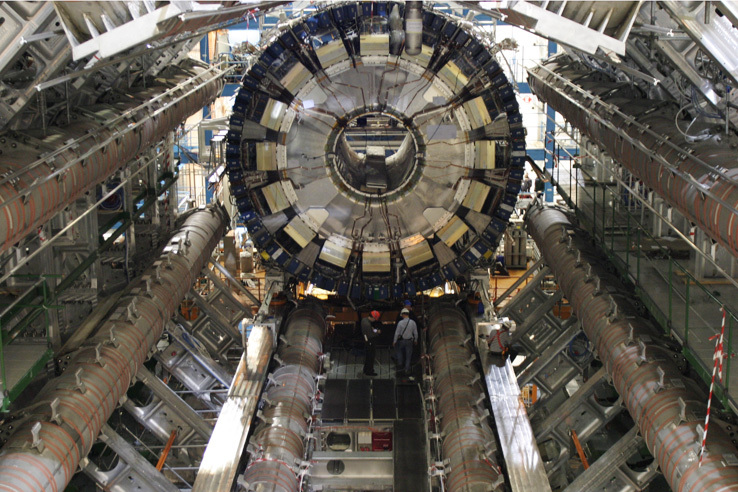
\includegraphics[width=0.7\textwidth]{tile.jpg}
\label{fig:detector:trt}
\caption{A photograph of the installation of the barrel tile calorimeter. Copyright CERN.}
\end{figure}

%%%%%%%%%%%%%%%% 


\section{Muon Spectrometer}


%%%%%%%%%%%%%%%%

\begin{figure}
\centering
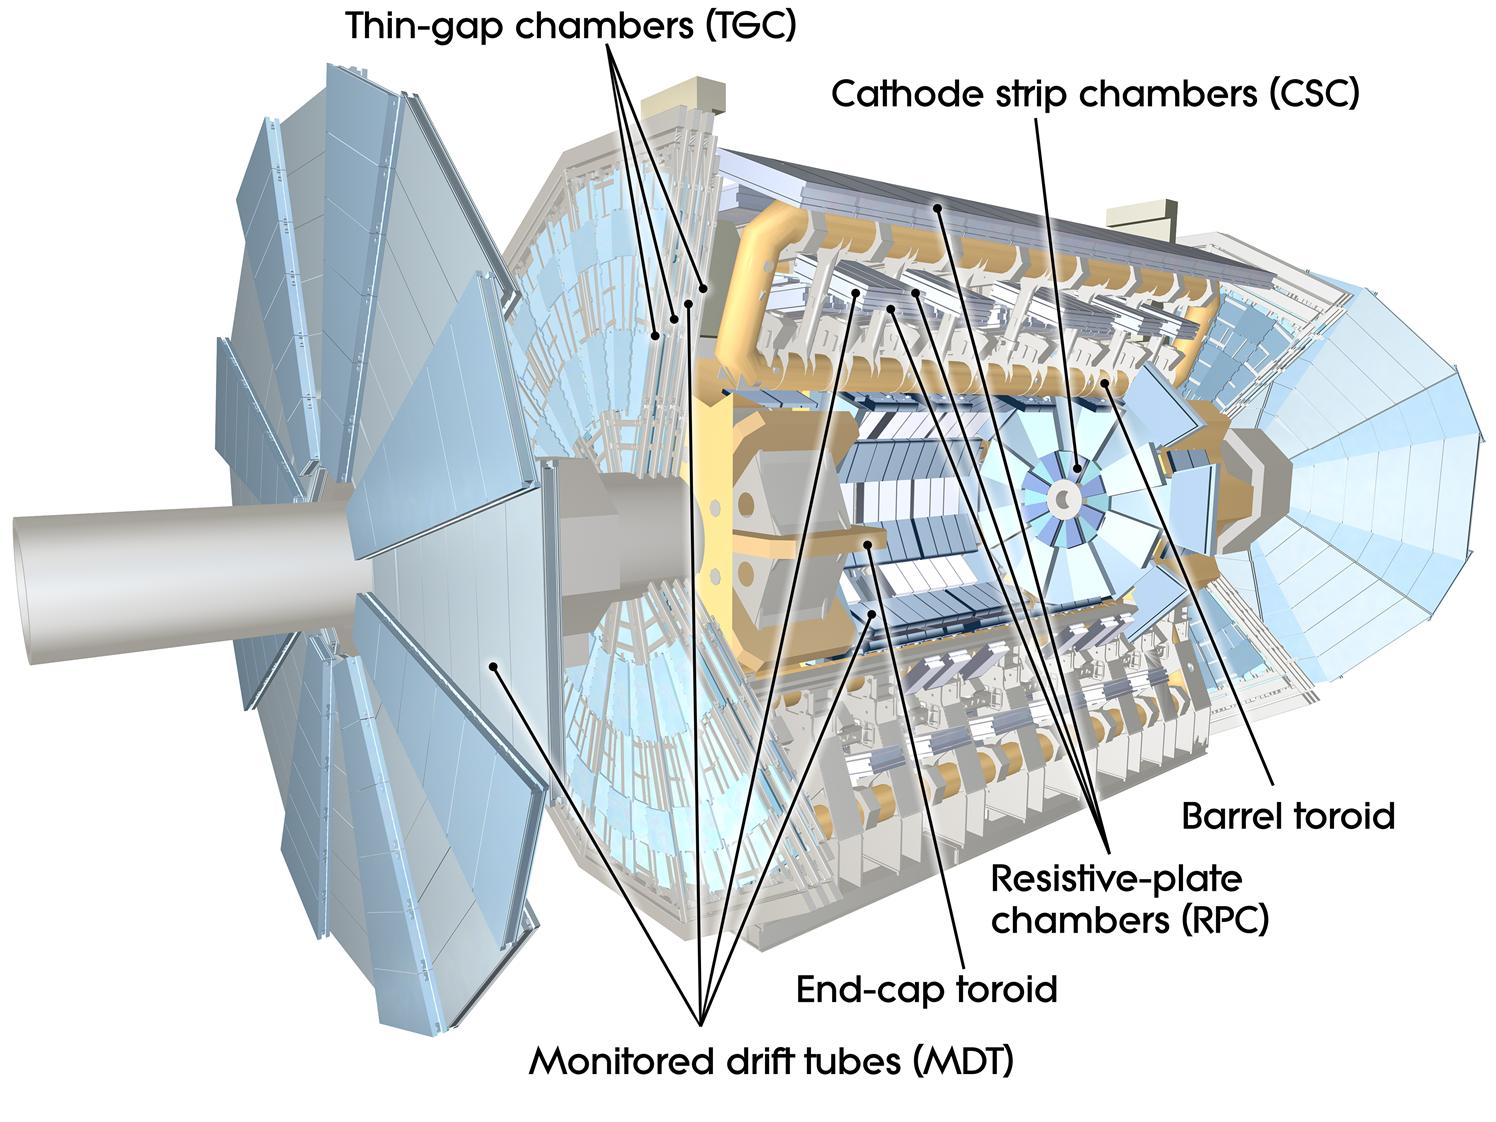
\includegraphics[width=0.7\textwidth]{muons.jpg}
\label{fig:detector:trt}
\caption{A computer generated image showing the locations of each of the muon spectrometer subsystems. Copyright CERN.}
\end{figure}

%%%%%%%%%%%%%%%% 

\section{Triggering}

\section{Data Quality}